\documentclass{standalone}
\usepackage{pgfplots}
\pgfplotsset{compat=newest}

\begin{document}
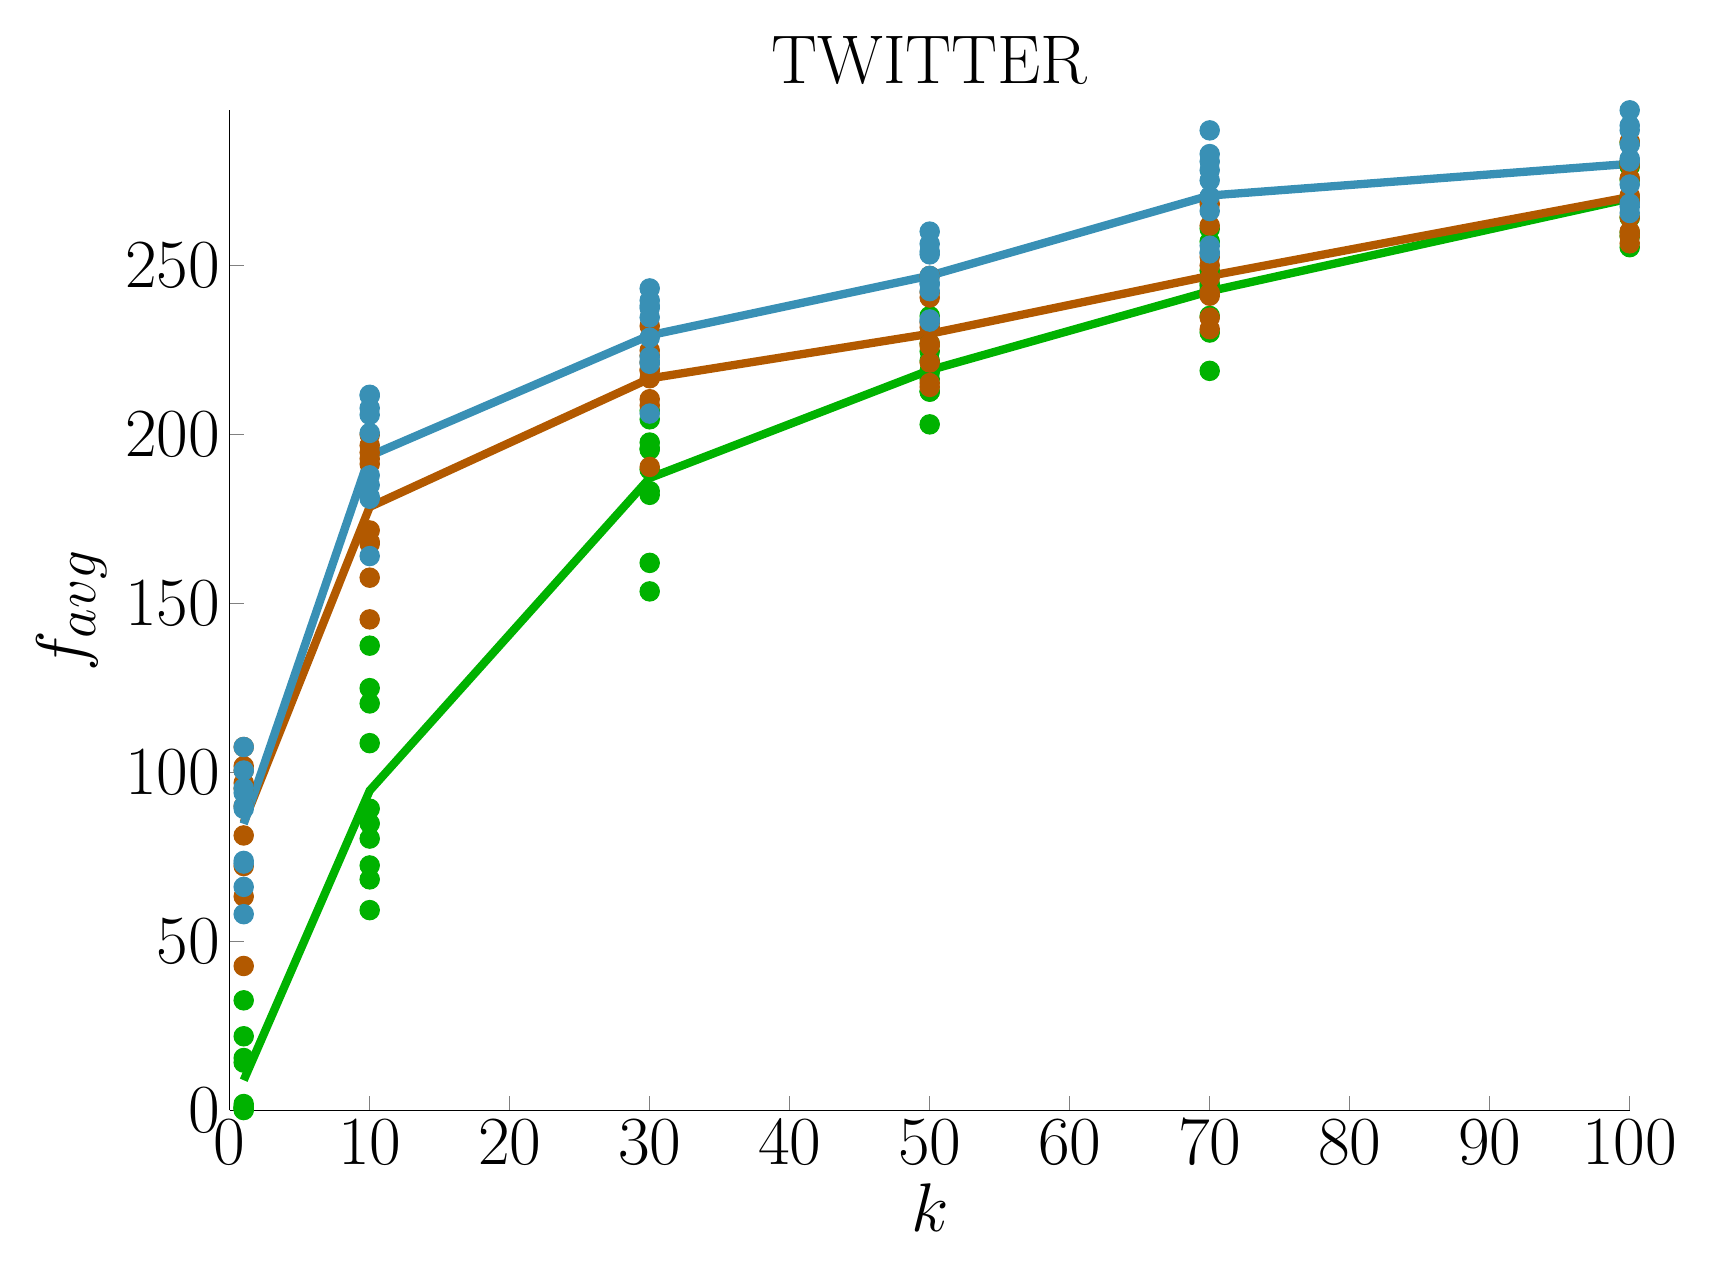
\begin{tikzpicture}

\begin{axis}[%
title style={font=\Huge},
title=TWITTER,
tick label style={font=\Huge},
label style={font=\Huge},
legend style={font=\Huge},
view={0}{90},
max space between ticks=50pt,
width=7in,
height=5in,
scale only axis,
xmin=0, xmax=100,
%xtick={0, 20, 40, 60, 80, 100},
xlabel={$k$},
ymin=0, ymax=296.0,
ylabel={$f_{avg}$},
major tick length=5pt,
axis lines*=left,
legend cell align=left,
clip=false]

\addplot [
only marks,
mark=*,
mark size=3.5pt,
color=green!70!black,
%solid,
%line width=2pt,
]
coordinates{
(1,0.08)(1,0.46)(1,0.74)(1,0.92)(1,0.96)(1,1.86)(1,14.12)(1,15.48)(1,21.92)(1,32.56)(10,59.26)(10,68.36)(10,72.48)(10,80.44)(10,84.9)(10,89.28)(10,108.68)(10,120.44)(10,124.96)(10,137.54)(30,153.6)(30,162.04)(30,182.18)(30,183.28)(30,189.64)(30,195.56)(30,195.98)(30,197.66)(30,204.54)(30,207.16)(50,203.04)(50,212.74)(50,212.74)(50,216.42)(50,218.5)(50,218.82)(50,221.86)(50,224.66)(50,226.94)(50,235.1)(70,218.88)(70,230.22)(70,235.14)(70,242.06)(70,242.94)(70,244.06)(70,244.64)(70,248.62)(70,257.14)(70,260.92)(100,255.48)(100,258.68)(100,259.76)(100,264.22)(100,268.98)(100,270.32)(100,275.38)(100,279.36)(100,280.5)(100,286.42)
};

\addplot [
only marks,
mark=*,
mark size=3.5pt,
color=orange!70!black,
%solid,
%line width=2pt,
]
coordinates{
(1,42.72)(1,63.3)(1,72.3)(1,81.36)(1,90.04)(1,95.26)(1,96.88)(1,100.58)(1,101.86)(1,107.54)(10,145.32)(10,157.66)(10,167.68)(10,168.22)(10,171.64)(10,191.3)(10,192.86)(10,194.66)(10,196.82)(10,199.96)(30,190.44)(30,208.68)(30,210.48)(30,216.7)(30,218.86)(30,219.28)(30,221.4)(30,223.38)(30,224.92)(30,232.16)(50,214.12)(50,215.26)(50,221.34)(50,226.26)(50,227.02)(50,231.78)(50,233.1)(50,240.58)(50,242.08)(50,246.98)(70,231.22)(70,234.64)(70,241.12)(70,241.82)(70,241.9)(70,246.34)(70,250.1)(70,252.58)(70,261.86)(70,268.26)(100,256.62)(100,258.86)(100,260.12)(100,264.42)(100,269.22)(100,270.72)(100,275.82)(100,279.96)(100,280.92)(100,286.7)
};

\addplot [
only marks,
mark=*,
mark size=3.5pt,
color=cyan!70!black,
%solid,
%line width=2pt,
]
coordinates{
(1,58.06)(1,66.14)(1,73.04)(1,73.82)(1,89.26)(1,90.04)(1,93.96)(1,95.38)(1,100.58)(1,107.54)(10,164.06)(10,181.02)(10,181.6)(10,185.06)(10,187.96)(10,200.5)(10,205.86)(10,207.84)(10,211.52)(10,211.8)(30,206.24)(30,220.96)(30,221.72)(30,223.04)(30,228.7)(30,234.7)(30,237.46)(30,238.16)(30,239.72)(30,243.28)(50,233.46)(50,234.1)(50,242.48)(50,244.52)(50,244.84)(50,246.98)(50,253.36)(50,254.2)(50,256.46)(50,260.1)(70,253.66)(70,253.96)(70,255.92)(70,266.18)(70,270.54)(70,275.26)(70,278.28)(70,280.84)(70,283.04)(70,290.06)(100,265.6)(100,267.48)(100,268.4)(100,274.04)(100,280.86)(100,281.64)(100,285.84)(100,290.12)(100,291.48)(100,296.0)
};
p
\addplot [
color=green!70!black,
solid,
line width=3pt
]
coordinates{
(1,8.91)(10,94.634)(30,187.164)(50,219.082)(70,242.462)(100,269.91)
};

\addplot [
color=orange!70!black,
solid,
line width=3pt
]
coordinates{
(1,85.184)(10,178.612)(30,216.63)(50,229.852)(70,246.984)(100,270.336)
};

\addplot [
color=cyan!70!black,
solid,
line width=3pt
]
coordinates{
(1,84.782)(10,193.722)(30,229.398)(50,247.05)(70,270.774)(100,280.146)
};


\end{axis}
\end{tikzpicture}
\end{document}
